\chapter{Descripci�n T�cnica}

Hemos utilizado una red multicapa, ya que permiten representar superficies de decisi�n no lineales. Debido a esto no se puede utilizar unidades lineales ya que solo permitir�an representar funciones lineales. Tampoco pudimos utilizar perceptrones porque su funci�n de salida es discontinua, no derivable y por lo tanto no se le puede aplicar el descenso del gradiente. Necesit�bamos una unidad que diese como salida una funci�n no lineal y que fuese derivable con respecto a las entradas.
Por eso utilizamos el sigmoide como unidad.

\begin{center}
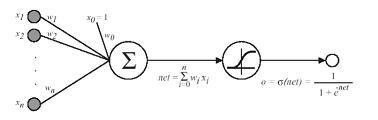
\includegraphics[scale=1]{red2.png} 
\end{center} 

La funci�n sigma $ \sigma(x) = \dfrac{1}{1 + e^{-x}} $   es no lineal y derivable $ \dfrac{d\sigma(x)}{dx} = \sigma(x) . (1 - \sigma(x)) $.
El descenso de gradiente se puede utilizar para entrenar:
\begin{itemize}
\item Una unidad sigmoide.
\item Una red multicapa de unidades sigmoides. Retropropagaci�n.
\end{itemize} 

La retropropagaci�n permite aprender los pesos para una red multicapa con un numero de unidades e interconexiones dado. Consideramos una red con m�ltiples unidades de salida, de forma que el error es la suma de los errores sobre todas las salidas. El espacio de hip�tesis viene dado por los valores posibles para los pesos de todas las unidades de red. Utilizamos el descenso de gradiente para encontrar una hip�tesis que minimice el error, el descenso utilizado es incremental, es decir, los pesos se actualizan despu�s de considerar cada ejemplo de entrenamiento en lugar de esperar a considerarlos todos. Es mas improbable que el descenso incremental caiga en un m�nimo local.

La secuencia de pasos utilizada en nuestro entrenamiento viene a ser esta:
\begin{itemize}
\item Crear la red. 
\item Se inicializan los pesos de la red con valores peque�os y aleatorios entre -0.05 y 0.05
\item Para una media de 30 iteraciones se realiza lo siguiente: De una lista de im�genes de entrenamiento se va cogiendo una a una y se cargan en la capa de entrada de la red, para esa imagen se calculan las capas, luego seg�n un objetivo se calculo el error cometido en la capa oculta y en la salida y respecto a estos errores se reajustan los pesos de las interconexiones.
\item Se realiza un prueba y una validaci�n con im�genes distintas a las del entrenamiento, para ver el porcentaje de error total cometido, si es aceptable se guarda en un archivo los pesos de la red entrenada, para que en la fase de reconocimiento de im�genes solo haya que realizar el calculo de capas.
\end{itemize} 	

Para cada unidad de salida k, se calcula su termino de error: $ \delta_{k} = O_{k} . (1 - O_{k}) . (t_{k} - O_{k}) $
Para cada unidad oculta h, se calcula su termino de error: $ \delta_{h} = O_{h} . (1 - O_{h}) . \Sigma (W_{kh} . \delta_{k}) $ , siendo k las salidas.
Se actualiza cada peso de la red $ W_{ji} = W_{ji} + \Delta (W_{ji}) $ donde $ \Delta (w_{ji}) = \eta .\delta_{j} .x_{ji} + \alpha .\Delta w_{ji}. (n-1) $. 
(t_{k} es la salida dada por ejemplo de entrenamiento para la unidad k. o_{t} es la salida generada por la red.)
La actualizaci�n de los pesos en la iteraci�n n depende de la actualizaci�n en n-1. El 2� termino de la ecuaci�n representa la cantidad de movimiento. Un s�mil f�sico seria una pelota que cae por la superficie de error, la cantidad de movimiento hace que la pelota tienda a mantener la misma direcci�n, con esto se intenta evitar que la pelota pare en un m�nimo local o que se pare en un llano.

Respecto el descenso del gradiente en el sigmoide:
Para el descenso incremental consideramos el cambio en los pesos inducido por cada ejemplo de entrenamiento $ \Delta w_{ji} = -\eta . \dfrac{\eth E_{d}}{\eth w_{ji}} $
donde el error sobre un ejemplo de entrenamiento viene dado por la suma de los errores en cada unidad de salida $ E_{d}(w) \equiv \frac{1}{2} . \Sigma (t_{k} - o_{k})^{2} $ , siendo k las salidas
La salida viene dada por $ net = \Sigma w_{i}.x_{i} $ , i=0..n y $ o = \sigma (net) = \dfrac{1}{1 + e^{-net}} $, aplicando la regla de la cadena $ \dfrac{\eth E_{d}}{\eth w_{ji}} = \dfrac{\eth E_{d}}{\eth net_{j}} . \dfrac{\eth net_{j}}{\eth w_{ji}} = \dfrac{\eth E_{d}}{\eth net_{j}} . x_{ji} $. Para calcular $ \dfrac{\eth E_{d}}{\eth net_{j}} $ distinguimos el caso de las unidades de salida y las ocultas.
Error en las unidades de salida $ \dfrac{\eth E_{d}}{\eth net_{j}} = -(t_{j} - o_{j}). o_{j} .(1 - o_{j}) $. Error en la unidades ocultas $ \dfrac{\eth E_{d}}{\eth net_{j}} = o_{j} . (1 - o_{j}) . \Sigma (-\delta_{k} . w_{kj})  $.

Para valores peque�os de los pesos (al principio del proceso) la red presenta una funci�n casi lineal donde es menos probable encontrar m�nimos locales. Cuando la funci�n es mas compleja (un punto mas avanzado del proceso) es de esperar que nos hayamos acercado tanto al m�nimo global que los m�nimo locales sean aceptables. Para garantizar que alcanzamos el m�nimo global utilizamos heur�sticas:
\begin{itemize}
\item A�adiendo cantidad de movimiento.
\item Utilizando descenso incremental.
\item Entrenar distintas redes con los mismos ejemplos, pero con distintos valores iniciales en los pesos.
\end{itemize} 

La capacidad expresiva de este tipo de red es bastante alta ya que:
\begin{itemize}
\item Cualquier funci�n booleana se puede representar con una red de dos capas.
\item Cualquier funci�n continua se puede aproximar con un error arbitrariamente peque�o por una red de dos capas.
\item Cualquier funci�n se puede aproximar con un error arbitrariamente peque�o por una red de tres capas (las dos ocultas de sigmoides y la de salida de unidades lineales).
\end{itemize} 

Respecto al sesgo inductivo:
El espacio de hip�tesis es continuo a diferencia de los espacios de hip�tesis de otros m�todos inductivos
Las redes neuronales realizan una interpolaci�n. Dados dos ejemplos positivos que no tienen ejemplos negativos entre ellos se tienden a etiquetar como positivos todos los puntos intermedios

